\documentclass[11pt,a4paper]{article}
\usepackage[margin=2.5cm]{geometry}
\usepackage{iftex}
\ifPDFTeX % pdfLaTeX (Overleaf default); XeTeX/tectonic needs none of this
  \usepackage[T1]{fontenc}
  \usepackage[utf8]{inputenc}
  \usepackage{lmodern}
\fi
\usepackage{textcomp}
\usepackage{booktabs}
\usepackage{graphicx}
\usepackage[hidelinks]{hyperref}
% repository layout: report/ next to results/; on Overleaf: put the PNGs in figures/
\graphicspath{{../results/figures/}{figures/}}
\emergencystretch=2em % lets lines with long file names break without overflowing

\newcommand{\eur}{\texteuro}
\newcommand{\obs}{\par\noindent\textit{Observation.} }
\newcommand{\interp}{\par\noindent\textit{Interpretation.} }

\begin{document}

\begin{center}
{\Large\bfseries Football ticket resale prices in the weeks before kickoff}\\[6pt]
Group G: Charles, Erdem, Chris, Liam, Gabriel\\
Data, Data Storage, Data Collection \quad--\quad 27.11.2026\\
Code and data: \url{https://github.com/GabDestal/data_storage_football_scraper}
\end{center}

\section{Question and data}

We ask how football ticket resale (asking) prices evolve in the weeks before a match, and what explains the differences between matches. Seat categories are a secondary question.

\textbf{Source.} Ticombo (ticombo.fr) is a ticket resale platform. Each match page embeds a JSON summary of its listings, for the match and for each seat category: lowest, average and highest asking price and tickets listed. There are no individual listings and no listing IDs. Our main measure is \texttt{listing\_startPrice}, the lowest asking price without fees: averages are pulled up by a few extreme listings, and the fee changed during collection (Section~2).

\textbf{Scope and collection.} The 100 Premier League and LaLiga matches kicking off 17.10--23.11.2026 (50 per league); 97 were on Ticombo (all 50 Premier League, 47 LaLiga). Fixtures, kickoffs and results come from the football-data.org API. A scheduled run requested each match page once a day (1 ticket, 4--8 seconds between requests): 5,485 requests, 5,484 successful, over 57 days from 27.09 to 23.11 (03.10 is missing). A day's prices cannot be collected again, so we kept all 5,463 raw pages (zipped, in Git LFS and a GitHub release).

\textbf{Legal checks.} We checked robots.txt and the terms on 27.09, before collecting; the screenshots in \texttt{docs/tos\_checks} were retaken on 26.11. Ticombo's robots.txt only disallows \texttt{/*/styleguide/}, \texttt{/*/buy\$} and \texttt{/*/userInfo/*}, and our scraper skips \texttt{/buy} URLs. Ticombo's terms (last updated August 2026) have no clause on robots, scrapers or automated access to the site (the only mention of bots concerns sellers buying tickets). The pages need no login and showed no captcha. We store no personal data. StubHub was rejected because its terms forbid ``any robot, spider, scraper or other automated means''; viagogo belongs to the same group and was rejected too.

\section{Cleaning}

\texttt{clean\_data.py} flags rows instead of deleting them, so every rule can be checked. Table~\ref{tab:cleaning} shows what each rule removes from the analysis.

\begin{table}[htbp]
\centering
\caption{From parsed snapshots to the analysis sample (\texttt{quality\_summary.json}).}
\label{tab:cleaning}
\begin{tabular}{lrr}
\toprule
Step & Snapshots & Matches \\
\midrule
Match snapshots parsed (one per match and day) & 5,435 & 97 \\
\quad taken at or after kickoff & $-$2,068 & \\
\quad second snapshot on the same day; kickoffs more than 1 day apart & 0; 0 & \\
Pre-kickoff snapshots & 3,367 & 97 \\
\quad no ticket listed & $-$124 & \\
\quad fee ratio outside 1.30--1.35 & $-$16 & \\
Snapshots with a usable price & 3,227 & 95 \\
\quad of which in the last 21 days before kickoff & 1,907 & 95 \\
\quad flagged top 1\% (above \eur 897.40), kept & 33 & 5 \\
\bottomrule
\end{tabular}
\end{table}

\textbf{Kickoffs} come from the final football-data.org run (24.11), which fixed placeholder LaLiga times; no Ticombo kickoff is more than one day away. \textbf{Days with no ticket listed} can still show an old ``from'' price, so they are flagged by tickets, not by a missing price, and kept for listed supply; two LaLiga matches never had a listing. \textbf{Fees:} the fee-included price is normally 1.30 times the base price, but from 04.11, 203 pre-kickoff snapshots of 27 matches show 1.35, so the fee-included price is only a robustness check. \textbf{Extreme prices:} 22 of the 33 top 1\% snapshots are El Cl\'asico (Barcelona--Real Madrid), a genuinely expensive match, not an error.

\textbf{Common window.} Trajectories use the last 21 days before kickoff. Collection started on 27.09, so the 17 matches of 17--18.10 start at day 19 or 20. We therefore index each match to its own median price 14--21 days before kickoff, a period every match has, instead of day 21.

\textbf{Seat categories.} The 26,060 category snapshots carry 230 raw labels that differ by stadium. \texttt{map\_categories.py} groups them with keyword rules (side, behind the goal, corner, premium, away). Categories describe 50.7\% of the listed tickets, so seat results stay secondary.

\section{Storage}

The clean data is stored in one SQLite file (\texttt{football.db}) with five normalised tables: \texttt{matches} (100 rows), \texttt{standings} (120), \texttt{event\_snapshots} (5,435), \texttt{seat\_categories} (230) and \texttt{category\_snapshots} (26,060). Primary keys are the natural keys; foreign keys link snapshots to matches and category rows to snapshots. Match information and seat groups are stored once, so they cannot become inconsistent. Flags are 0/1 columns the analysis filters on.

Table~\ref{tab:storage} compares three formats on the same query (average lowest price per league and day in the 21-day window). All three return the same result. At our size every format is fast. We chose SQLite because it enforces types and keys in a single file that every group member can query. Parquet is the smallest and would suit a much larger, read-only dataset.

\begin{table}[htbp]
\centering
\caption{Storage formats (\texttt{compare\_storage.py}, median of 20 runs).}
\label{tab:storage}
\begin{tabular}{lrrrccc}
\toprule
Format & Files & Size (MB) & Query (ms) & Types & Keys & Match info repeated \\
\midrule
CSV + pandas & 3 & 8.82 & 14.2 & no & no & yes \\
SQLite & 1 & 5.51 & 1.2 & yes & yes & no \\
Parquet + DuckDB & 5 & 0.39 & 10.8 & yes & no & no \\
\bottomrule
\end{tabular}
\end{table}

\textbf{Correction to peer review 2.} The review said foreign keys would have prevented ``294 event snapshots with no category rows''. A foreign key prevents orphan children, that is, a category row whose snapshot does not exist; there are 0 in \texttt{football.db}. It cannot force a snapshot to have categories. In the final data, 434 snapshots have no category rows and they are not errors: 177 are pages with no listings, and 257 have listings for which Ticombo published no per-category breakdown.

\section{Results}

\textbf{Method.} Trajectories divide each match's lowest price by its median 14--21 days before kickoff (index 100). The fixed-effects (FE) regression is $\log(\mathrm{price}) \sim$ day bin $+$ match dummies, with standard errors clustered by match; bins are whole days before kickoff (0--2, 3--6, 7--13, 14--21 as reference). The match dummies absorb each match's price level, so the bins measure how the price moves within a match. A4 is one OLS across matches with robust (HC1) standard errors. Team ranks at kickoff are rebuilt from the official results of matches finished before each kickoff (football-data.org); the rebuilt tables match all six standings files saved during collection. All outputs are in \texttt{results/}.

\subsection*{A0 Data overview}
\obs 97 of 100 matches have a Ticombo page, with a median of 33 pre-kickoff days. In the example match Liverpool--Manchester United (Figure~\ref{fig:a0}) the median lowest price goes from \eur 324 (14--21 days) to \eur 358 (0--2 days).
\interp Coverage is almost complete in both leagues, but a single match is noisy and can go against the average, so we compare medians over many matches.

\begin{figure}[htbp]
\centering
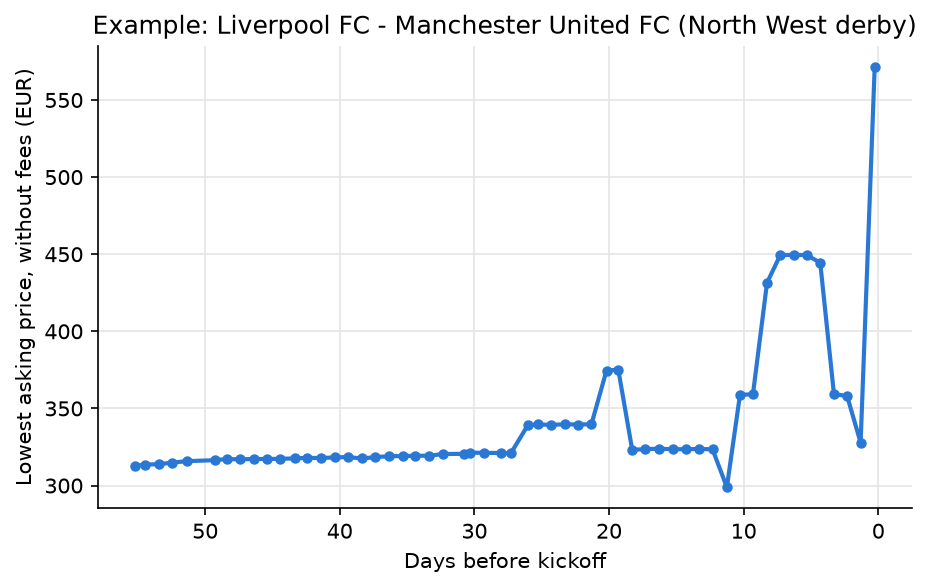
\includegraphics[width=0.48\textwidth]{a0_example_match.png}
\caption{Example match Liverpool--Manchester United (North West derby): lowest asking price without fees on every pre-kickoff day.}
\label{fig:a0}
\end{figure}

\subsection*{A1 How prices move}
\obs In the median match the price index is 66 (Premier League) and 82 (LaLiga) in the last 3 days (Figure~\ref{fig:a1}). In the FE model the lowest price is 23.0\% lower at 0--2 days than at 14--21 days (Table~\ref{tab:fe}). Our October preliminary estimate was $-19$\%.
\interp Within a match, the cheapest ticket on offer gets cheaper as kickoff approaches, mostly in the last week and more in the Premier League. This fits sellers cutting prices before the ticket loses its value, but also new cheap listings or expensive ones being withdrawn. Without listing IDs we cannot tell these apart.

\begin{figure}[htbp]
\centering
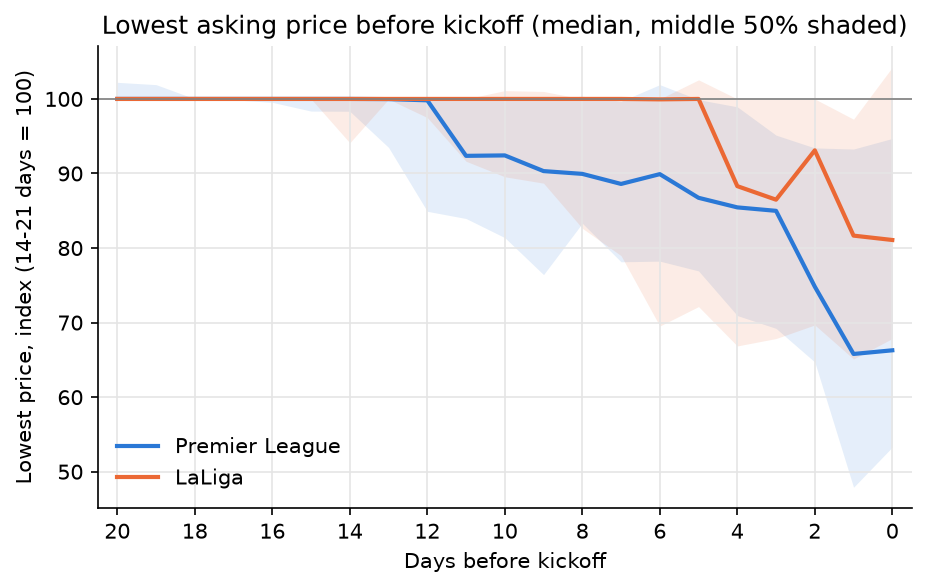
\includegraphics[width=0.68\textwidth]{a1_trajectory_by_league.png}
\caption{Lowest asking price before kickoff, indexed to each match's 14--21 day median (median and middle 50\%).}
\label{fig:a1}
\end{figure}

\begin{table}[htbp]
\centering
\caption{FE regression: change in the lowest price compared with 14--21 days before kickoff, in \% (95\% CI).}
\label{tab:fe}
\begin{tabular}{lccc}
\toprule
Days before kickoff & All & Premier League & LaLiga \\
\midrule
7--13 & $-5.3$ [$-10.7$, 0.5] & $-4.9$ [$-14.3$, 5.5] & $-5.7$ [$-10.2$, $-0.9$] \\
3--6 & $-13.4$ [$-18.4$, $-8.1$] & $-13.4$ [$-20.9$, $-5.3$] & $-13.4$ [$-19.9$, $-6.4$] \\
0--2 & $-23.0$ [$-29.0$, $-16.5$] & $-28.9$ [$-37.5$, $-19.3$] & $-16.1$ [$-23.2$, $-8.4$] \\
\midrule
Snapshots & 1,907 & 997 & 910 \\
Matches (= clusters) & 95 & 50 & 45 \\
\bottomrule
\end{tabular}
\end{table}

\subsection*{A2 Different paths}
\obs Comparing 0--2 days with 14--21 days (93 matches with both), the lowest price falls by more than 5\% in 72\% of matches, stays within $\pm$5\% in 14\% and rises in 14\%. With a $\pm$10\% band, 61\% fall. In the last 3 days the index is 95 for the cheapest third of matches and 67 for the most expensive third.
\interp A falling price is the typical path, not a rule. The drop is concentrated in the more expensive matches; part of this may be regression to the mean.

\subsection*{A3 Listed supply}
\obs The number of tickets listed is flat until the last week, then reaches index 78 in both leagues over the last 3 days (Premier League 70, LaLiga 35 on the last day). Day-to-day changes in tickets listed and in the lowest price have a correlation of $-0.06$ (1,779 day pairs, 95 matches).
\interp Listed supply shrinks just before kickoff, but its daily changes are almost unrelated to price changes. A ticket can leave the listings because it was bought or withdrawn; we cannot tell which, so we only speak of listed supply.

\subsection*{A4 Differences between matches}
\obs Table~\ref{tab:a4}: weekend matches are 32.6\% more expensive ($p=0.002$; October estimate: $+40$\%). Each place further down the table for the better team goes with $-3.1$\%, and derbies with $+88.3$\% (6 derbies). Without the top 1\% prices, El Cl\'asico and Hull City--Brighton drop out: the weekend coefficient stays, while best rank and derby fall to $p=0.069$.
\interp The weekend association is the only one robust to dropping the top 1\% prices; best rank and derby depend on a few extreme matches. With 12 weekday matches, 6 derbies and $R^2=0.17$, these are descriptive associations, not causal effects.

\begin{table}[htbp]
\centering
\caption{OLS of the log median lowest price 7--14 days before kickoff: effect in \% (p-value, HC1).}
\label{tab:a4}
\begin{tabular}{lcc}
\toprule
 & All matches & Without top 1\% prices \\
\midrule
Weekend & $+32.6$ (0.002) & $+31.4$ (0.002) \\
Best rank of the two teams, $+1$ place & $-3.1$ (0.023) & $-2.2$ (0.069) \\
Rank gap, $+1$ place & $-1.4$ (0.36) & $-1.3$ (0.38) \\
Derby & $+88.3$ (0.030) & $+57.7$ (0.069) \\
Premier League (vs LaLiga) & $-8.8$ (0.44) & $-10.5$ (0.31) \\
\midrule
Matches & 94 & 92 \\
\bottomrule
\end{tabular}
\end{table}

\subsection*{A5 Seat categories (secondary)}
\obs The median category price 14--21 days before kickoff is \eur 547 for premium seats, \eur 344 on the side and \eur 288 behind the goal. At 0--2 days their index is 86, 93 and 90; away sections (23 matches) end at 83. Corner seats (4 matches) end at 110.
\interp Premium seats cost most, but all main groups end below their earlier level by a similar amount: we find no sign that premium seats fall more than the away end. The drop is smaller than in A1 because a category price averages all its listings.

\subsection*{A6 Robustness}
\obs The 0--2 day drop is $-22.4$\% with fees included, $-24.2$\% without the top 1\% prices and $-24.3$\% with all pre-kickoff days. In that full window, prices more than 21 days before kickoff are 14.6\% above the 14--21 day level.
\interp The last-days drop keeps its sign and size under every choice, so it does not depend on the fee, the extreme prices or the window.

\section{Limitations}
\begin{itemize}
\item Asking prices on one platform, with no transactions and no listing IDs: we cannot tell whether the lowest price falls because sellers cut prices, cheaper tickets are listed or expensive ones leave. Other resale sites and official exchanges are not covered.
\item One snapshot per day, between about 05:00 and 21:00 UTC; 03.10 is missing. The interrupted 06.10 run (05:53 UTC) was redone at 06:19 and its 49 pages were deleted. 28 pages of a partial, unlogged 22.10 run (08:07 UTC) duplicate the logged 21:04 run and are not parsed. Neither incident loses a snapshot day.
\item Seat categories describe 50.7\% of the listed tickets. Ranks at kickoff ignore LaLiga's head-to-head tie-break, but our rebuilt tables match all six saved standings files.
\item A4 rests on 94 matches (12 on weekdays, 6 derbies) with $R^2=0.17$. Thin markets can set a match's price level: Hull City--Brighton had 4 tickets at \eur 1,500 for six days.
\end{itemize}

\section{Changes after the peer reviews}

R1 and R2 are peer reviews 1 and 2.

\noindent
\begin{tabular}{p{0.32\textwidth}p{0.62\textwidth}}
\toprule
Comment & What we changed \\
\midrule
Daily run, backup, gap check & Scheduled daily run; raw pages in Git LFS and a release; \texttt{parse.py} prints the pages per day. \\
Extreme prices distort averages (R2) & Lowest price as main measure; medians; top 1\% flagged, robustness check. \\
Common window (R1) & Last 21 days, each match indexed to its 14--21 day median. \\
Empty reference files (R2) & Face values dropped; seat groups mapped automatically (230 labels); 26 derby pairs. \\
Database, redundancy (R2) & SQLite with 5 normalised tables; foreign key claim corrected (434 = 177 + 257, 0 orphans). \\
No data exploration (R2) & A0: coverage table and one example match. \\
Listing IDs (R2, question 8) & There are none; tickets listed are read as listed supply only. \\
Round 1 plan: weekly standings, fee-included price & Ranks rebuilt from results (standings saved only 3 times); base price as main measure (fee rose from 1.30 to 1.35 on 04.11). \\
\bottomrule
\end{tabular}

\end{document}
